\documentclass[12pt]{article}
\usepackage{geometry}
\usepackage{xcolor}
\usepackage{listings}
\usepackage{graphicx}
\geometry{
	top = 20mm,
	left = 25mm,
	right = 25mm,
	bottom = 20mm
}
\geometry{a4paper}
%\renewcommand{\familydefault}{\sfdefault}
\renewcommand{\baselinestretch}{1.3}

\definecolor{mGreen}{rgb}{0,0.6,0}
\definecolor{mGray}{rgb}{0.5,0.5,0.5}
\definecolor{mPurple}{rgb}{0.58,0,0.82}
\definecolor{mRed}{rgb}{1, 0, 0}
\definecolor{backgroundColour}{rgb}{0.95,0.95,0.92}

\lstdefinestyle{CStyle}{
	commentstyle=\color{mGreen},
	keywordstyle=\color{mPurple},
	numberstyle=\tiny\color{mGray},
	stringstyle=\color{mGreen},
	basicstyle=\ttfamily\footnotesize,
	emph = {},
	emphstyle=\color{red},
	breakatwhitespace=false,         
	breaklines=true,                 
	captionpos=b,                    
	keepspaces=true,                 
	numbers=left,                    
	numbersep=10pt,                  
	showspaces=false,                
	showstringspaces=false,
	showtabs=false,                  
	tabsize=4,
	language=C++,
}

\lstdefinestyle{PyStyle}{
	commentstyle=\color{mGreen},
	keywordstyle=\color{mPurple},
	numberstyle=\tiny\color{mGray},
	stringstyle=\color{mGreen},
	basicstyle=\ttfamily\footnotesize,
	emph = {},
	emphstyle=\color{red},
	breakatwhitespace=false,         
	breaklines=true,                 
	captionpos=b,                    
	keepspaces=true,                 
	numbers=left,                    
	numbersep=-10pt,                  
	showspaces=false,                
	showstringspaces=false,
	showtabs=false,                  
	tabsize=4,
	language=Python,
}

%opening
\title{\sffamily Algorithms: Order Statistics Red Black Tree}
\author{2017-18570 Sungchan Yi\\Dept. of Computer Science and Engineering}
\date{May 15th, 2019}
\begin{document} 

\maketitle
\tableofcontents

\section{Introduction}
In this homework, we implement an \textbf{order statistic red black tree} with C++ language using data structure augmentation. Compared to normal red black trees, order statistics tree will contain an additional field \textit{size} in each node $v$, which keeps track of the number of nodes in the subtree with root $v$. Additionally, we implement a checker program for the correctness for the implemented data structure and operations. The implemented tree should support the following operations:
\begin{itemize}
	\item \textsc{OS-Insert}$(T, x)$: Insert $x$ into $T$. If $x$ already exists in $T$, return 0. Otherwise, return $x$.
	\item \textsc{OS-Delete}$(T, x)$: Delete $x$ from $T$. If $x$ is not in $T$, return 0. Otherwise, return $x$.
	\item \textsc{OS-Select}$(T, i)$: Select the $i$-th smallest key from $T$ and return it. If $i$ is greater than the number of keys currently in $T$, return 0.
	\item \textsc{OS-Rank}$(T, x)$: Return the rank of $x$ if $x$ is in $T$. Otherwise, return 0.
\end{itemize}
The following are the restrictions on given inputs.
\begin{itemize}
	\item Each operation will be denoted as I, D, S, R respectively.
	\item $1\leq x \leq 9999$.
	\item Input will be given in the form ``[Character representing the operation] [x]".
\end{itemize}

\section{Implementation}
The basic operations required for the tree was implemented as the same way in the textbook, so we omit it here.

\subsection{Checker}
To check the correctness, we implement a checker program. The basic idea is to use a \texttt{vector<int> vec} to keep track of the set of integers given as input.
\begin{itemize}
	\item \texttt{check\_insert(int x)} will traverse \texttt{vec} and check if \texttt{x} is already in the vector. If it is, immediately return \texttt{0}. If it is not found, \texttt{push\_back x} and return \texttt{x}.
\begin{lstlisting}[style=Cstyle]
int check_insert(int x) {
	for(auto v : vec) {
		if(v == x) return 0;
	}
	vec.push_back(x);
	return x;
}
\end{lstlisting} 
	\item \texttt{check\_delete(int x)} will traverse \texttt{vec} and check if \texttt{x} is already in the vector. If it is, swap it with the last element of \texttt{vec}, \texttt{pop\_back}, and return \texttt{x}. If it is not found, return \texttt{0}.
\begin{lstlisting}[style=Cstyle]
int check_delete(int x) {
	for(int i = 0; i < vec.size(); ++i) {
		if(x == vec[i]) {
			int tmp = vec[vec.size() - 1];
			vec[vec.size() - 1] = x;
			vec[i] = tmp;
			vec.pop_back();
			return x;
		}
	}
	return 0;
}
\end{lstlisting}

\item \texttt{check\_select(int x)} will first check if \texttt{x} is less then the size of \texttt{vec}. If it is, sort the vector and return \texttt{vec[x - 1]}. Else, return \texttt{0}.
\begin{lstlisting}[style=Cstyle]
int check_select(int x) {
	if(x <= vec.size()) {
		sort(vec.begin(), vec.end());
		return vec[x - 1];
	} else return 0;
}
\end{lstlisting}

\item \texttt{check\_rank(int x)} will sort the vector and then traverse the list. If \texttt{x} is found, return the (index of \texttt{x}) + 1. If it is not found, return \texttt{0}.
\begin{lstlisting}[style=Cstyle]
int check_rank(int x) {
	sort(vec.begin(), vec.end());
	for(int i = 0; i < vec.size(); ++i) {
		if(vec[i] == x) return i + 1;
	}
	return 0;
}

\end{lstlisting}
\end{itemize}
And here is the checker code. Interpret \texttt{opt\_seq} and perform \texttt{check\_[op]}, then compare it with the given \texttt{out\_seq}. If the result doesn't match in any point in time, return \texttt{false}.
\begin{lstlisting}[style=Cstyle]
bool check(int opt_seq[], int in_seq[], int out_seq[], int n) {
	string str = "";
	for(int i = 0; i < n; ++i) {
		if(opt_seq[i] == 0) {
			if(check_insert(in_seq[i]) != out_seq[i]) {
				printf("%d: WA on I %d\n", i, in_seq[i]);
				return false;
			}
		} else if(opt_seq[i] == 1) {
			if(check_delete(in_seq[i]) != out_seq[i]) {
				printf("%d: WA on D %d\n", i, in_seq[i]);
				return false;
			}
		} else if(opt_seq[i] == 2) {
			if(check_select(in_seq[i]) != out_seq[i]) {
				printf("%d: WA on S %d\n", i, in_seq[i]);
				return false;
			}
		} else if(opt_seq[i] == 3) {
			if(check_rank(in_seq[i]) != out_seq[i]) {
				printf("%d: WA on R %d\n", i, in_seq[i]);
				return false;
			}
		}
	}
	return true;
}
\end{lstlisting}

\section{Experiments}
Here is how the test was done.
\begin{itemize}
	\item Test environment
	\begin{itemize}
		\item OS: Ubuntu 18.04.2 LTS
		\item CPU: Intel® Core™ i5-6200U CPU @ 2.30GHz $\times$ 4
		\item RAM: 8GB  
	\end{itemize}
	\item Test Case Generator (Python)\\
	We keep the numbers small so that the numbers generated in the test will overlap easily, which will cause more operations to return some value other than 0.
	\begin{lstlisting}[style=PyStyle]
	from random import randint
	
	# Select random element from list
	def rndselect(list):
		idx = randint(0, len(list) - 1)
		return list[idx]
	
	# Number of Test Cases
	N = 100000
	
	# Operation set
	op_set = ['I', 'D', 'R', 'S']
	
	# Numbers
	num = [str(i) for i in range(1, 100)]
	
	# Create input text file
	f = open('tests/input', "w")
	
	# Write to test file
	f.write(str(N) + "\n")
	for i in range(N):
		f.write(rndselect(op_set))
		f.write(' ')
		f.write(rndselect(num))
		f.write('\n')
	f.close()
	\end{lstlisting}
	\item Checker Code\\
	This is the checker code I implemented, to check the correctness of my implementation. An helper function \texttt{printSideways} was used to examine the tree structure easily.
	\begin{lstlisting}[style=Cstyle]
	#include <cstdio>
	#include "hw2_cpp.h"
	#define N 101010
	
	extern Tree tree; // Tree defined in hw2_cpp.h
	
	int opt_seq[N], in_seq[N], out_seq[N];
	
	int main() {
		string str = "";
	
		freopen("./tests/input", "r", stdin);
		string op;
		int x, t;
		cin >> t;
		for(int i = 0; i < t; ++i) {
			cin >> op >> x;
			in_seq[i] = x;
			printf("%d. %c %d : ", i + 1, op[0], x);
			if(op[0] == 'I') {
				opt_seq[i] = 0;
				out_seq[i] = os_insert(x);
			} else if(op[0] == 'D') {
				opt_seq[i] = 1;
				out_seq[i] = os_delete(x);
			} else if(op[0] == 'S') {
				opt_seq[i] = 2;
				out_seq[i] = os_select(x);
			} else if(op[0] == 'R') {
				opt_seq[i] = 3;
				out_seq[i] = os_rank(x);
			}
			printf("%d\n", out_seq[i]);
			tree.printSideways(tree.getRoot(), str);
		}
		
		puts("Checking...");
		if(check(opt_seq, in_seq, out_seq, t)) puts("correct");
		else puts("incorrect");
	}
\end{lstlisting}
	\item \texttt{printSideways} function\\
	Prints the \textit{data} and \textit{size} of each node, with colors embedded.
\begin{lstlisting}[style=Cstyle]
void Tree::printSideways(Node* node, string& indent) {
	string str = indent + "        ";
	if(node != NIL) {
		printSideways(node -> right, str);
		if(node -> color == RED) {
			cout << indent;
			printf("\033[1;31m(%d / %d)\033[0m\n", node -> data, node -> size);
		} else {
			cout << indent;
			printf("\033[1;30m(%d / %d)\033[0m\n", node -> data, node -> size);
		}
		printSideways(node -> left, str);
	}
}
\end{lstlisting}
	\item Test case generator code was saved to \texttt{tester.py}, the checker code was saved to \texttt{os\_test.cpp}.
	\begin{itemize}
		\item Generate Test: \texttt{python3 tester.py}
		\item Compile: \texttt{g++ os\_test.cpp -o test}
		\item Run: \texttt{./test}
	\end{itemize}
\end{itemize}

\subsection{Test Case \#1}
I tried a small test case first, with small numbers.\\
10\quad
I 3\quad
I 13\quad
I 2\quad
S 1\quad
R 6\quad
R 5\quad
D 10\quad
I 17\quad
I 7\quad
I 8\quad\\
Here is the structure of the tree after each operation.
Each node is represented by $(key / size)$. The leftmost node is the root, and by each column, the nodes in the next level are shown.
\pagebreak
\begin{figure}[h!]
	\begin{center}
		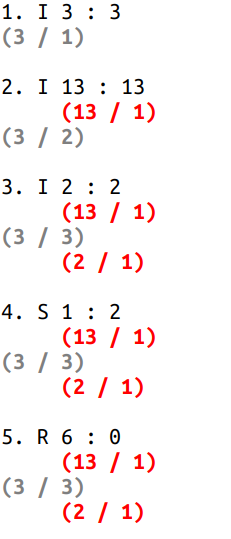
\includegraphics[width=4.5cm, height=10cm]{pic/test1-1.png}
		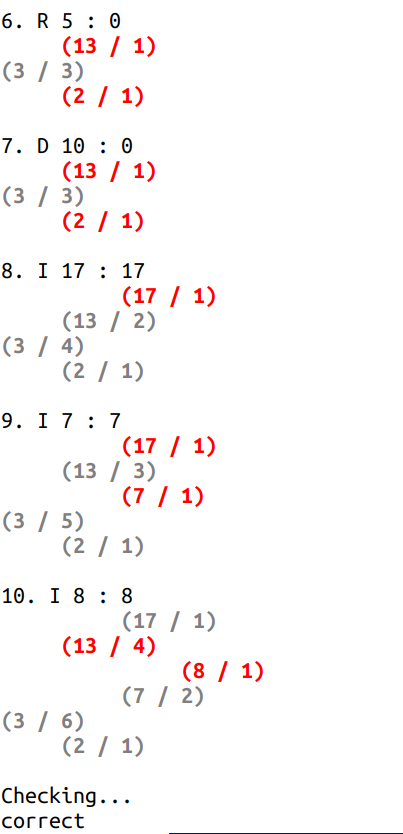
\includegraphics[width=7cm, height=14cm]{pic/test1-2.png}
		\caption{Result of Test 1}
	\end{center}

\end{figure}
\subsection{Test Case \#2}
For the second case, I tried a case with size 30.\\
30\quad
I 9\quad
I 1\quad
S 12\quad
R 19\quad
R 14\quad
S 6\quad
S 11\quad
R 9\quad
I 3\quad
D 10\quad
S 5\quad
S 17\quad
D 13\quad
I 19\quad
I 19\quad
S 6\quad
R 3\quad
S 7\quad
I 1\quad
S 10\quad
R 8\quad
I 3\quad
I 10\quad
I 2\quad
I 11\quad
I 15\quad
I 13\quad
I 16\quad
R 15\quad
D 6\\
\pagebreak
\begin{figure}[h!]
	\begin{center}
		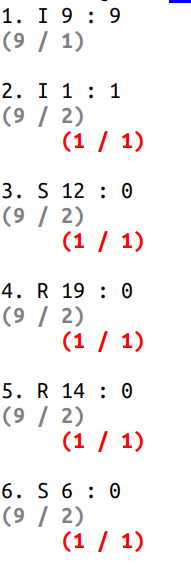
\includegraphics[width=4cm, height=10cm]{pic/test2-1.png}
		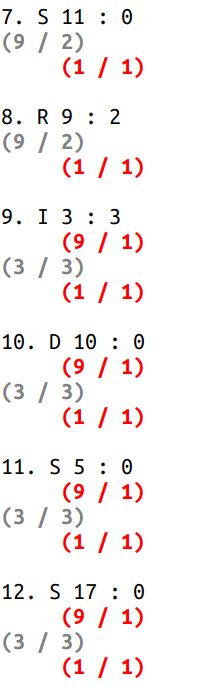
\includegraphics[width=4cm, height=10cm]{pic/test2-2.png}
		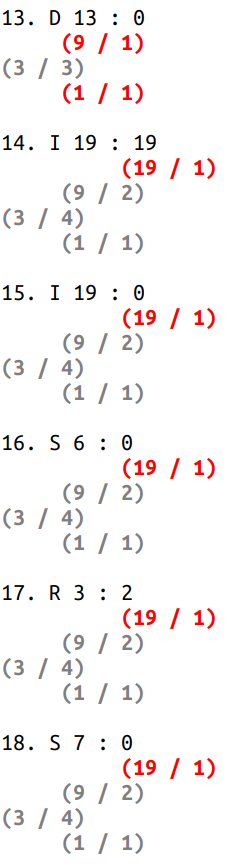
\includegraphics[width=4cm, height=10cm]{pic/test2-3.png}
		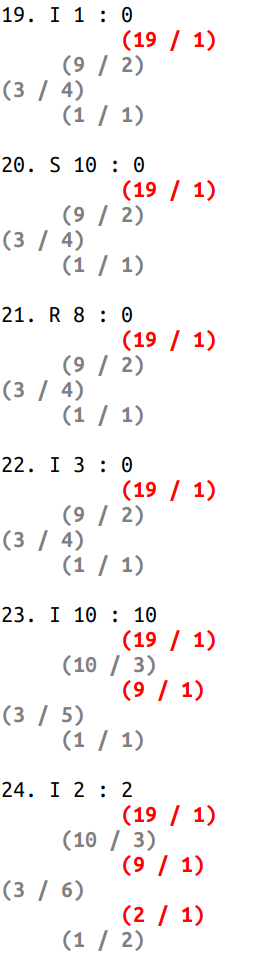
\includegraphics[width=4cm, height=12cm]{pic/test2-4.png}
		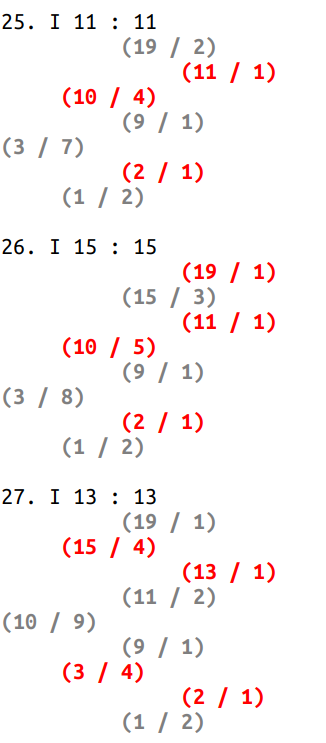
\includegraphics[width=4cm, height=12cm]{pic/test2-5.png}
		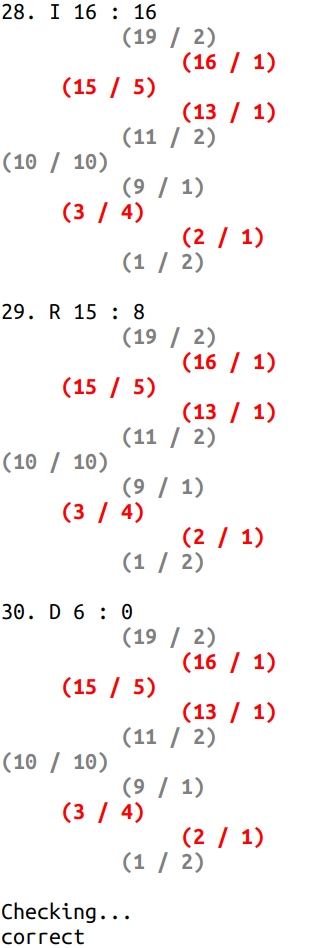
\includegraphics[width=4cm, height=12cm]{pic/test2-6.png}
		\caption{Result of Test 2}
	\end{center}
\end{figure}
\pagebreak
\\
I ran many other cases, up to $100000$ operations. They were all correct.
\section{Conclusion}
In this homework, I learned how to augment data structures to contain additional information, that will help me retrieve particular information. With the augmented data structure, the additional field could be calculated in $O(1)$ time, since it only needs the information from left/right child. In total, \texttt{rank}, \texttt{select} takes $O(\log n)$ time with the order statistics tree, since the height of a red black tree is at most $O(\log n)$.
\end{document}
